\documentclass[9pt,twocolumn,twoside,lineno]{gsajnl}
% Use the documentclass option 'lineno' to view line numbers

\usepackage{epstopdf}
\usepackage{indentfirst}
\usepackage{booktabs}
\usepackage{multirow}
\usepackage{graphicx}
\usepackage[table,xcdraw]{xcolor}

\articletype{inv} 

\runningtitle{Heart rate variability for analysis of human well-being} % For use in the footer

\title{Heart rate variability for analysis of human well-being}

\author[]{Andrey Khomutov, Polina Volos}
%\author[]{Polina Volos}


\begin{abstract}
This work uses HRV data from four Subjects with the aim to find the healthiest. HRV data is processed with the help of the \textit{Pyhrv} library to extract various metrics based on \textit{time-domain} and \textit{frequency-domain} measurements. These metrics are analysed with linkage to normal values and correlation with such parameters as \textit{Stress} and \textit{Well-being}, which would provide the determination of the healthiest patient.

\end{abstract}

\begin{document}

\maketitle
\thispagestyle{firststyle}
%\slugnote
%\firstpagefootnote
\vspace{-13pt}% Only used for adjusting extra space in the left column of the first page

\section{Introduction}
There are many metrics for HRV data analysis, and they are divided into 3 types according to the type of analysis:
\textit{time-domain}, \textit{frequency-domain}, and \textit{non-linear} measurements. So on, there is a diversity of metrics for each of the 3 types [\ref{metrics}]. 

It is worth mentioning that there are 2 types of HRV data: \textit{Short-term} measurements (based on ~5 min of ECG data) and \textit{Twenty-four} hour measurements. Since the time of taking ECG data for the given four Subjects varied from 20 to 30 minutes, it is obvious that our initial data should be considered Short-term. In such a case, it has been shown that non-linear measurements should not be used for stress analysis [\ref{fine_stress}]. 


\section{Methods}
It was decided to use the following time-domain metrics for stress analysis: Root mean square of successive RR interval
differences (RMSSD), Standard deviation of NN intervals (SDNN) and Percentage of successive RR intervals that differ by
more than 20 ms (pNN20). At the same time, we will use low-frequency band (LF), TP (= HF + LF + VLF) and LF/HF of the frequency-domain type which is recommended in the reference article [\ref{given_article}].

To extract the metrics, the file data was processed in Python using the \textit{pyhrv} library (figure \ref{fig1}). Frequency-domain metrics were obtained with the use of Welch's method (figure \ref{fig2}). 


\section{Results}
The final results are presented in table \ref{table1}. 

Initially, standard values were found for SDNN (50 $\pm$ 16 ms), RMSSD (42 $\pm$ 15 ms), LF (519 $\pm$ 291 $ms^2$), TP (1000 $\pm$ 3500)[10] and LF/HF (2.8 $\pm$ 2.6) in healthy adults [\ref{healthy_adults}]. According to these data, patients 1 (RMSSD) and 4 (LF) do not fall under the standard values and may have health problems. 

Further, we began to study in more detail the dependence of the values of these parameters on various states of human health. We found out that : 

1) subjects with low RMSSD values (poor vagus-mediated HRV) tended to have higher SUDEP-7 scores (higher risk for Sudden unexplained death in epilepsy) [\ref{epilepsy}], 

2) reduced SDNN, RMSSD, and pNN20 were independent markers for LQTS(+) (Long QT-Syndrome patients that are at risk of arrhythmias and seizures) across various physiological states [\ref{LQTS}], 

3) the reduction of SDNN, rMSSD metrics was confirmed  with stress condition [\ref{table}],

4) the pNN20 parameter is highly negatively correlated to stress and depression and to some extent positively to well-being [\ref{table}], 

5) SDNN, RMSSD, LF and HF were significantly lower in patients with high 10-year CHD (coronary heart disease) risk [\ref{chd}], 

6) SDNN, RMSSD, pNN20, LF significantly decreased in the order of normal coronary artery, non-obstructive CAD (coronary artery disease), and angiographic CAD [\ref{cad}]. 


\begin{figure*}[b] 

    \centering
    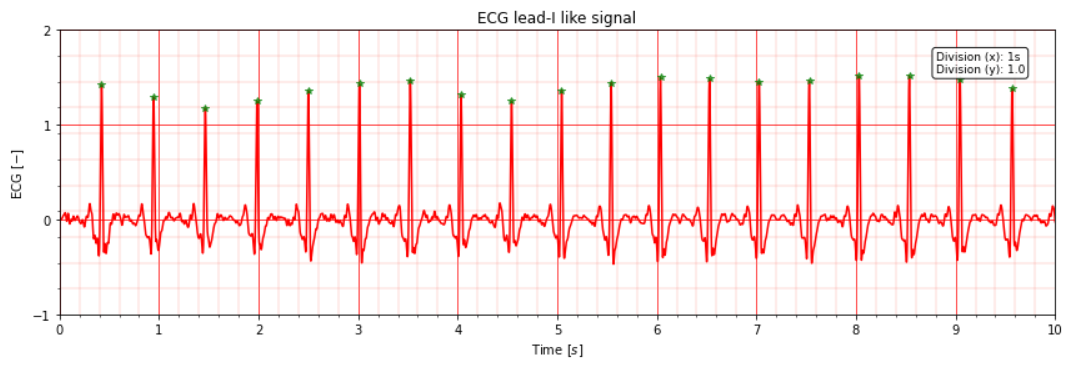
\includegraphics[scale=0.5]{ecg.png}
    \caption{\centering Sample ECG signal of Subject 1}
    
 \label{fig1}
\end{figure*} 

\begin{figure*}[b] 

    \centering
    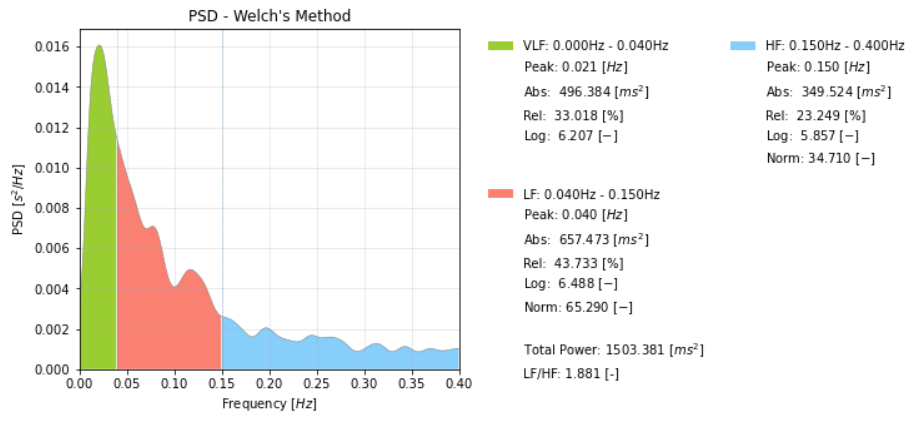
\includegraphics[scale=0.56]{psd.png}
    \caption{\centering Sample Power spectral density of Subject 1}
    
 \label{fig2}
\end{figure*} 


\section{Discussion}
Although general trends between HRV metrics and well-being are determined firmly, we have to mention that you could easily find contradictory figures (especially for the normal values) in different articles due to age, athleticism, sex and other parameters of the test group.

Nevertheless, we have made a conclusion that the 4th patient should be considered the best at well-being. The only exceptional metric is LF, which is higher than the norms. Yet, LF/HF values are fine. Subject 4 has the highest TP, SDNN, RMSSD and pNN20 values (which is the most similar to the norms [\ref{pnn20}]. Again, all these metrics have a positive correlation with general well-being and a negative correlation with subjective measures of perceived stress [\ref{table}].

The most unhealthy patient is Subject 1, who seems to be suffering from stress.

\section{References}

\begin{enumerate}

\item \label{metrics}
Shaffer F, Ginsberg JP. An Overview of Heart Rate Variability Metrics and Norms. Front Public Healh. 2017;5(September):1–17. 

\item \label{fine_stress}
Pereira T, Almeida PR, Cunha JPS, Aguiar A. Heart rate variability metrics for fine-grained stress level assessment. Comput Methods Programs Biomed. 2017;148:71–80. 

\item \label{given_article}
https://vc.ru/tech/121021-kak-rasschityvayutsya-pokazateli-stressa-i-energii-v-fitnes-gadzhetah-analiz-variabelnosti-serdechnogo-ritma

\item \label{healthy_adults}
Nunan D, Sandercock GRH, Brodie DA. A quantitative systematic review of normal values for short-term heart rate variability in healthy adults. PACE - Pacing Clin Electrophysiol. 2010;33(11):1407–17. 

\item \label{epilepsy}
Epps J, Gordon S, Gornbein J, Ph D, Harper RM, Ph D. RMSSD, a Measure of Heart Rate Variability, Is Associated With Risk Factors For SUDEP: The SUDEP-7 Inventory Christopher.Pdf. 2011;19(1):78–81. 

\item \label{LQTS}
DeMaria N, Selmi A, Kashtan S, Xia X, Wang M, Zareba W, et al. Autonomic and Cardiac Repolarization Lability in Long QT Syndrome Patients. Auton Neurosci Basic Clin [Internet]. 2020;229(August):102723. Available from: https://doi.org/10.1016/j.autneu.2020.102723

\item \label{table}
Trimmel M. Relationship of Heart Rate Variability (HRV) Parameters Including pNNxx With the Subjective Experience of Stress, Depression, Well-Being, and Every-Day Trait Moods (TRIM-T): A Pilot Study. Ergon Open J. 2015;8(1):32–7. 

\item \label{chd}
Yoo CS, Lee K, Yi SH, Kim JS, Kim HC. Association of heart rate variability with the framingham risk score in healthy adults. Korean J Fam Med. 2011;32(6):334–40.

\item \label{cad}
Li HR, Lu TM, Cheng HM, Lu DY, Chiou CW, Chuang SY, et al. Additive value of heart rate variability in predicting obstructive coronary artery disease beyond framingham risk. Circ J. 2016;80(2):494–501. 

\item \label{pnn20}
Corrales MM, Torres B de la C, Esquivel AG, Salazar MAG, Naranjo Orellana J. Normal values of heart rate variability at rest in a young, healthy and active Mexican population. Health (Irvine Calif). 2012;04(07):377–85. 

\end{enumerate}


\begin{table}[h]
\centering
\begin{tabular}{|
>{\columncolor[HTML]{FFFFFF}}c |
>{\columncolor[HTML]{FFFFFF}}c |
>{\columncolor[HTML]{FFFFFF}}c |
>{\columncolor[HTML]{FFFFFF}}c |
>{\columncolor[HTML]{FFFFFF}}c |
>{\columncolor[HTML]{FFFFFF}}c |
>{\columncolor[HTML]{FFFFFF}}c |}
\hline
\textbackslash{} & TP {[}ms\textasciicircum{}2{]} & LF {[}ms\textasciicircum{}2{]} & LF/HF & SDNN {[}ms{]} & RMSSD {[}ms{]} & pnn20 {[}\%{]} \\ \hline
Subject 1        & 1376                           & 547                            & 3,83  & 42,9          & 21,7           & 9,3            \\ \hline
Subject 2        & 1503                           & 657                            & 1,88  & 51,6          & 38,6           & 6,6            \\ \hline
Subject 3        & 1936                           & 719                            & 0,99  & 59,5          & 50,5           & 13,8           \\ \hline
Subject 4        & 2930                           & 1201                           & 1,17  & 64,5          & 56,1           & 18,6           \\ \hline
\end{tabular}
\caption{\centering Chosen metrics for each subject}
\label{table1}
\end{table}


\end{document}